% 使用 LuaLaTeX 或 XeLaTeX 编译：
%   latexmk -lualatex -shell-escape ttt_training_overview.tex
\documentclass[tikz,border=10pt]{standalone}
\usepackage{fontspec}
\usepackage{xcolor}
\usetikzlibrary{arrows.meta,backgrounds,calc,fit,positioning,shadows.blur}

\definecolor{ink}{HTML}{172033}
\definecolor{blue}{HTML}{DCEEFF}
\definecolor{mint}{HTML}{DDF7EE}
\definecolor{gold}{HTML}{FFF0C2}
\definecolor{rose}{HTML}{FFE0E8}
\definecolor{violet}{HTML}{E9DFFF}
\definecolor{line}{HTML}{59708A}

\tikzset{
  stage/.style={
    rounded corners=7pt,
    minimum width=30mm,
    minimum height=17mm,
    align=center,
    text=ink,
    font=\sffamily\small,
    draw=line!65,
    line width=.55pt,
    blur shadow={shadow blur steps=5,shadow xshift=1pt,shadow yshift=-1pt,opacity=.14},
  },
  flow/.style={-{Latex[length=3mm]},line width=.9pt,draw=line!85},
  note/.style={font=\sffamily\scriptsize\itshape,text=ink!75,align=center},
}

\begin{document}
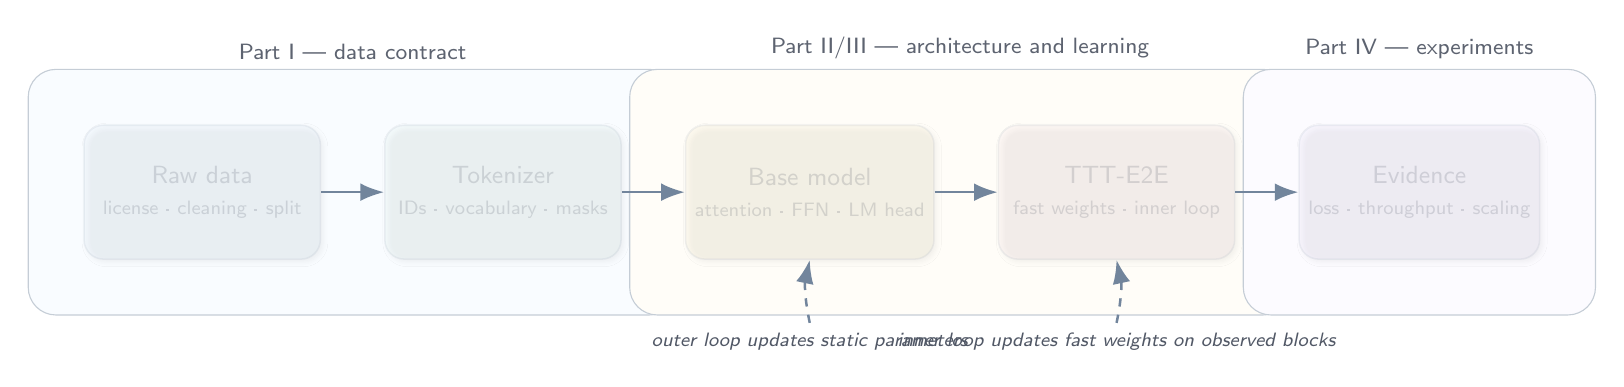
\begin{tikzpicture}[node distance=11mm and 8mm]
  \node[stage,fill=blue] (data) {Raw data\\\scriptsize license · cleaning · split};
  \node[stage,fill=mint,right=of data] (tokens) {Tokenizer\\\scriptsize IDs · vocabulary · masks};
  \node[stage,fill=gold,right=of tokens] (model) {Base model\\\scriptsize attention · FFN · LM head};
  \node[stage,fill=rose,right=of model] (ttt) {TTT-E2E\\\scriptsize fast weights · inner loop};
  \node[stage,fill=violet,right=of ttt] (evidence) {Evidence\\\scriptsize loss · throughput · scaling};

  \draw[flow] (data) -- (tokens);
  \draw[flow] (tokens) -- (model);
  \draw[flow] (model) -- (ttt);
  \draw[flow] (ttt) -- (evidence);

  \node[note,below=8mm of model] (outer) {outer loop updates static parameters};
  \node[note,below=8mm of ttt] (inner) {inner loop updates fast weights on observed blocks};
  \draw[flow,dashed] (outer.north) to[bend left=12] (model.south);
  \draw[flow,dashed] (inner.north) to[bend right=12] (ttt.south);

  \begin{scope}[on background layer]
    \node[draw=line!35,rounded corners=10pt,fit=(data)(tokens),inner sep=7mm,
      fill=blue!18,label={[font=\sffamily\footnotesize,text=ink!70]above:Part I — data contract}](data-group) {};
    \node[draw=line!35,rounded corners=10pt,fit=(model)(ttt),inner sep=7mm,
      fill=gold!12,label={[font=\sffamily\footnotesize,text=ink!70]above:Part II/III — architecture and learning}](model-group) {};
    \node[draw=line!35,rounded corners=10pt,fit=(evidence),inner sep=7mm,
      fill=violet!12,label={[font=\sffamily\footnotesize,text=ink!70]above:Part IV — experiments}](evidence-group) {};
  \end{scope}
\end{tikzpicture}
\end{document}
